\subsection{コンセプト}
今回作成するライブラリのコンセプトを以下に示す.

\begin{itemize}
 \item 対象者
       \begin{itemize}
	\item Androidアプリケーション開発初学者
       \end{itemize}
 \item 想定している使用目的
       \begin{itemize}
	\item 中・高生等を対象にしたセミナー
	\item Computer Graphics(CG)の授業や実験
	\item 企業等での3DCGを用いたAndroidプログラミングの学習
       \end{itemize}
 \item ライブラリの特徴
       \begin{itemize}
	\item 関数名や変数名を明瞭化
	\item 役割ごとにクラスを分け,各クラスの役割を明瞭化
	\item 拡張しやすい構成にする
	\item MainActivity\footnote{Androidアプリケーションを実行した時,一番最初に実行されるメソッド}はできるだけ最小限の構成に
       \end{itemize}
\end{itemize}

%\vspace{5pt}
\subsection{開発環境}

%\vspace{5pt}
\subsubsection{Android開発環境の現状}
現在,Androidアプリケーションの開発環境は以下の二つが主流である.
\begin{itemize}
 \item Eclipse\cite{Eclipse}
       \begin{itemize}
	\item Javaをはじめとするいくつかの言語に対応している統合開発環境である.Androidが登場してすぐの頃はEclipseでの開発が主流だった.
       \end{itemize}
 \item AndroidStudio\cite{AndroidStudio}
       \begin{itemize}
	\item Androidを開発しているGoogle社が提供しているAndroid統合開発環境である.初期のAndroidStudioは動作が不安定だった為しばらくはEclipseが使われていたが,最近はアップデートを繰り返し安定性が増してきている.
       \end{itemize}
       現在はEclipseからAndroidStudioに移りつつあると言える.しかし依然Eclipseで開発をする人が多い事も事実である.
\end{itemize}

\newpage
現状を踏まえて以下の環境で開発する事にした.
\begin{itemize}
 \item OS : Mac OS X Yosemite\cite{Yosemite}
       \begin{itemize}
	\item 動作の安定性,今後iOS版\footnote{iOSではSwiftと言われる言語を使用しており,開発は今の所Macでないと不可能である}の開発をする可能性などを考慮し,Mac miniを使用した.
       \end{itemize}
 \item 開発環境 : AndroidStudio 2.2.2
       \begin{itemize}
	\item 近年の開発環境の遷移を踏まえて,これからのスタンダードと考えられるため選択した.
       \end{itemize}
 \item 使用ライブラリ : ARToolKit version 5.3.1
       \begin{itemize}
	\item Androidの最新バージョンに対応している他,様々なプラットフォームに対応している為今後の展開を踏まえ選択した.
       \end{itemize}
 \item 実行端末 : Nexus 9\cite{Nexus9}
       \begin{itemize}
	\item Android 7.0 が動作するNexus 9 をARアプリケーションの実行端末として使用した.
       \end{itemize}
\end{itemize}

%\vspace{5pt}
\subsection{構造}
構造の明瞭化を図る為クラスを以下のように分割し,利用者が使用するクラス,ライブラリに格納できないクラスを除き全てライブラリに格納する.クラス図をFig.\ref{fig:class}に示す.またライブラリ化する事によって改変によるエラーを防ぎ,明瞭なコードになるよう促す.

%\vspace{5pt}
\subsubsection{Appモジュール}

\begin{itemize}
 \item MainActivity
       \begin{itemize}
	\item 簡易化する為,親クラスを変更しSetupを呼び出すだけとなっている.
       \end{itemize}
 \item Setup
       \begin{itemize}
	\item ここではライブラリに格納できない設定を行うクラスである.初学者には難しい設定や変更する必要のないメソッド等が格納されている為,ライブラリと共に提供されるクラスである.使用者は提供されたSetupクラスに指定の変更を加え,MainActivityと同じパッケージに入れるだけで実装が完了する.
       \end{itemize}
 \item AR
       \begin{itemize}
	\item 実際にARで表示したい物体の設定をするクラスである.簡易化を図る為,表示できるのはBoxのみである.Boxの大きさ,色,位置,角度,対応するARマーカーを登録するクラスで,使用者はここを変更する事で様々な変化を作る事ができる.
       \end{itemize}
\end{itemize}

%\vspace{5pt}
\subsubsection{ライブラリ}

\begin{itemize}
 \item Draw
       \begin{itemize}
	\item ARマーカの検出,及びBoxの表示をする処理が入っている.複数のマーカに反応させる場合や時間が経つにつれて変化を起こしたい場合,ここの処理を変更しないといけない.
       \end{itemize}
 \item ARSimpleApplication
       \begin{itemize}
	\item ARToolKitライブラリを使用する際にAppモジュールに追加しないといけなかったが,ライブラリ内に移動する事で処理の明瞭化を図る.
       \end{itemize}
 \item Cube
       \begin{itemize}
	\item 与えられた情報から色情報付きのBoxを生成するクラスである.ここを変更する事でBox以外の物体を表示できるが,今回のコンセプトと異なる為ライブラリ内に格納しBoxのみを表示するライブラリとした.
       \end{itemize}
\end{itemize}

その他,拡張現実感を実現する為のクラスが多々あるが,全てARToolKitから提供されている物である.

\begin{figure}[tb]
\centering
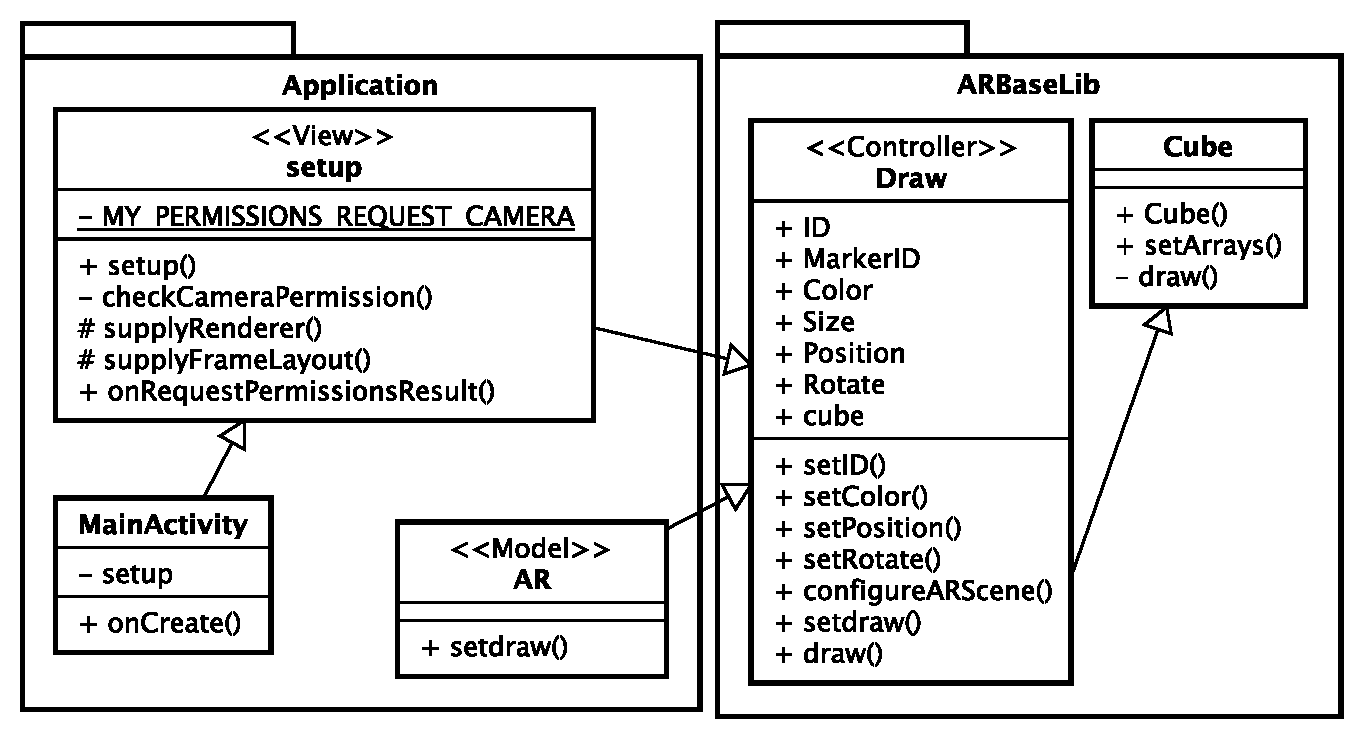
\includegraphics[width=12cm]{fig/android.pdf}
\caption{Class diagram}
\label{fig:class}
\end{figure}


